%! TEX program = pdflatex

\documentclass[oneside,solution]{tmpl}

\usepackage[utf8]{inputenc}
\usepackage[english,ukrainian]{babel}
\usepackage{float}

\title{Контрольна робота}
\author{Захаров Дмитро}
\studentID{МП-31}
\instructor{Ігнатович С.Ю.}
\date{\today}
\duedate{23:59 30 квітня, 2024}
\assignno{1}
\semester{Весняний семестр 2024}
\mainproblem{Контрольна Робота}

\begin{document}

\maketitle

% \startsolution[print]

\problem{Біфуркації.}

\hspace{20px}\textbf{Умова.} Нарисуйте фазові портрети наступних систем:
\begin{equation}
    (a): \begin{cases}
        \dot{x} = \mu x - x^2 \\
        \dot{y} = y
    \end{cases}, \; \; (b): \begin{cases}
        \dot{x} = \mu - x^2 \\
        \dot{y} = y
    \end{cases},
\end{equation}

де $\mu$ -- числовий параметр. Для кожної системи розгляньте три випадки: коли параметр $\mu$ додатний, дорівнює нулю і від'ємний. Опишіть, як змінюється фазовий портрет системи, коли параметр $\mu$ ``проходить через нуль''.

\textbf{Розв'язання.} Розглянемо пункти (а) і (б) окремо.

\textbf{Пункт (а).} Насправді, біфуркації стосуються лише першого рівняння, а друге рівняння системи потрібно для кращої геометричної інтерпретації і наочності, оскільки таким чином ми зможемо дати класифікацію точок на портреті в $\mathbb{R}^2$. Також, легко побачити, що для усіх $y(0):=y_0 \neq 0$, точка буде віддалятись на $\pm\infty$ від вісі $Ox$ по $y$ координаті в залежності від знаку $y_0$. Отже, сконцетруємось саме на першому рівнянні системи. Також одразу знайдемо точки спокою: це $(0,0)$ та $(\mu,0)$, проте вони вироджуються у одну точку у випадку $\mu=0$. Тому природньо розглянути такі випадки:

\textit{Випадок 1. $\mu > 0$.} Будемо дивитись на поведінку системи в залежності від початкової умови $x(0)=x_0$. Якщо $x_0<0$, то швидкість буде від'ємною, а тому точка буде віддалятись на $-\infty$ ліворуч. Якщо $x_0 \in (0,\mu)$, то швидкість буде додатною і тому точка буде наближатись до $x=\mu$. Нарешті, при $x>\mu$ швидкість від'ємна і точка буде також наближатись до $x=\mu$. Отже маємо стійку точку $x=\mu$ та нестійку $x=0$. Якщо додати друге рівняння $\dot{y} = y$, то для $(x,y)=(\mu,0)$ отримаємо сідло, а для $(x,y)=(0,0)$ -- нестійкий вузол.

\textit{Випадок 2. $\mu=0$.} Тоді рівняння перетворюється на $\dot{x} = -x^2$ -- тут єдина точка спокою $x=0$, що є напівстійкою -- праворуч від $x=0$ точка буде асимптотично наближатись до $x=0$, а ось для $x<0$, точка буде віддалятись на $-\infty$. Якщо додати ще друге рівняння $\dot{y}=y$, то це буде відповідати нестійкому вузлу ліворуч і сідлу праворуч від $x=0$.

\textit{Випадок 3. $\mu<0$.} Він є аналогічним випадку 1, проте тут вже точка $x=\mu$ є нестійкою, а $x=0$ -- стійкою, оскільки тепер точка $x=\mu$ знаходиться лівіше за $x=0$. Класифікація в $\mathbb{R}^2$ також зміниться відповідно: тепер $(x,y)=(0,0)$ є сідлом, а $x=(\mu,0)$ -- нестійким вузлом.

Спробуємо отримати ту саму класифікацію точок на $\mathbb{R}^2$, але вже лінеаризувавши систему:
\begin{equation}
    f(x,y) = \begin{bmatrix}\mu x-x^2 \\ y \end{bmatrix}, \;\; \boldsymbol{J}(x,y) = \frac{\partial f}{\partial (x,y)} = \begin{bmatrix}
        \frac{\partial f_x}{\partial x} & \frac{\partial f_x}{\partial y} \\
        \frac{\partial f_y}{\partial x} & \frac{\partial f_y}{\partial y}
    \end{bmatrix} = \begin{bmatrix}
        \mu - 2x & 0 \\
        0 & 1
    \end{bmatrix}
\end{equation}

Вважаємо $\mu \neq 0$. Тоді в точці $(0,0)$ маємо $\boldsymbol{J}(0,0) = \begin{bmatrix}
    \mu & 0 \\ 0 & 1
\end{bmatrix}$. Добре видно, що це відповідає двом власним значенням: $\lambda_1=\mu, \lambda_2 = 1$. Бачимо, що в залежності від знаку $\mu$, в нас або два власних значення додатні, або різних знаків. Отже, якщо $\mu > 0$, то $\lambda_1,\lambda_2>0$ -- нестійкий вузол. Якщо ж $\mu<0$, то $\lambda_1 < 0 < \lambda_2$ і тоді перед нами сідло. 

В точці спокою $(\mu,0)$ маємо Якобіан $\boldsymbol{J}(\mu,0) = \begin{bmatrix}
    -\mu & 0 \\ 0 & 1
\end{bmatrix}$, де власні значення $\lambda_1=-\mu,\lambda_2=1$. Тут ситуація симетрична: якщо $\mu>0$, то власні значення різних знаків $\implies$ перед нами сідло, якщо ж $\mu<0$, то маємо нестійкий вузол.

Отже, маємо ту саму класифікацію. Перевіримо її за допомогою малюнку (код буде наведений в самому кінці для обох пунктів) -- див. Рис. \ref{fig:problem_1a}. Дійсно бачимо, що для $\mu = -1$ зліва для точки $(-1,0)$ маємо нестійкий вузол, а праворуч для $(0,0)$ -- сідло. Для $\mu=0$ зліва від точки маємо вузол, праворуч -- сідло. Для $\mu=1$ та $\mu=2$ маємо для $(0, 0)$ нестійкий вузол, а для $(\mu, 0)$ -- сідло. Дійсно збіглося з нашим аналізом.

\begin{figure}
    \centering
    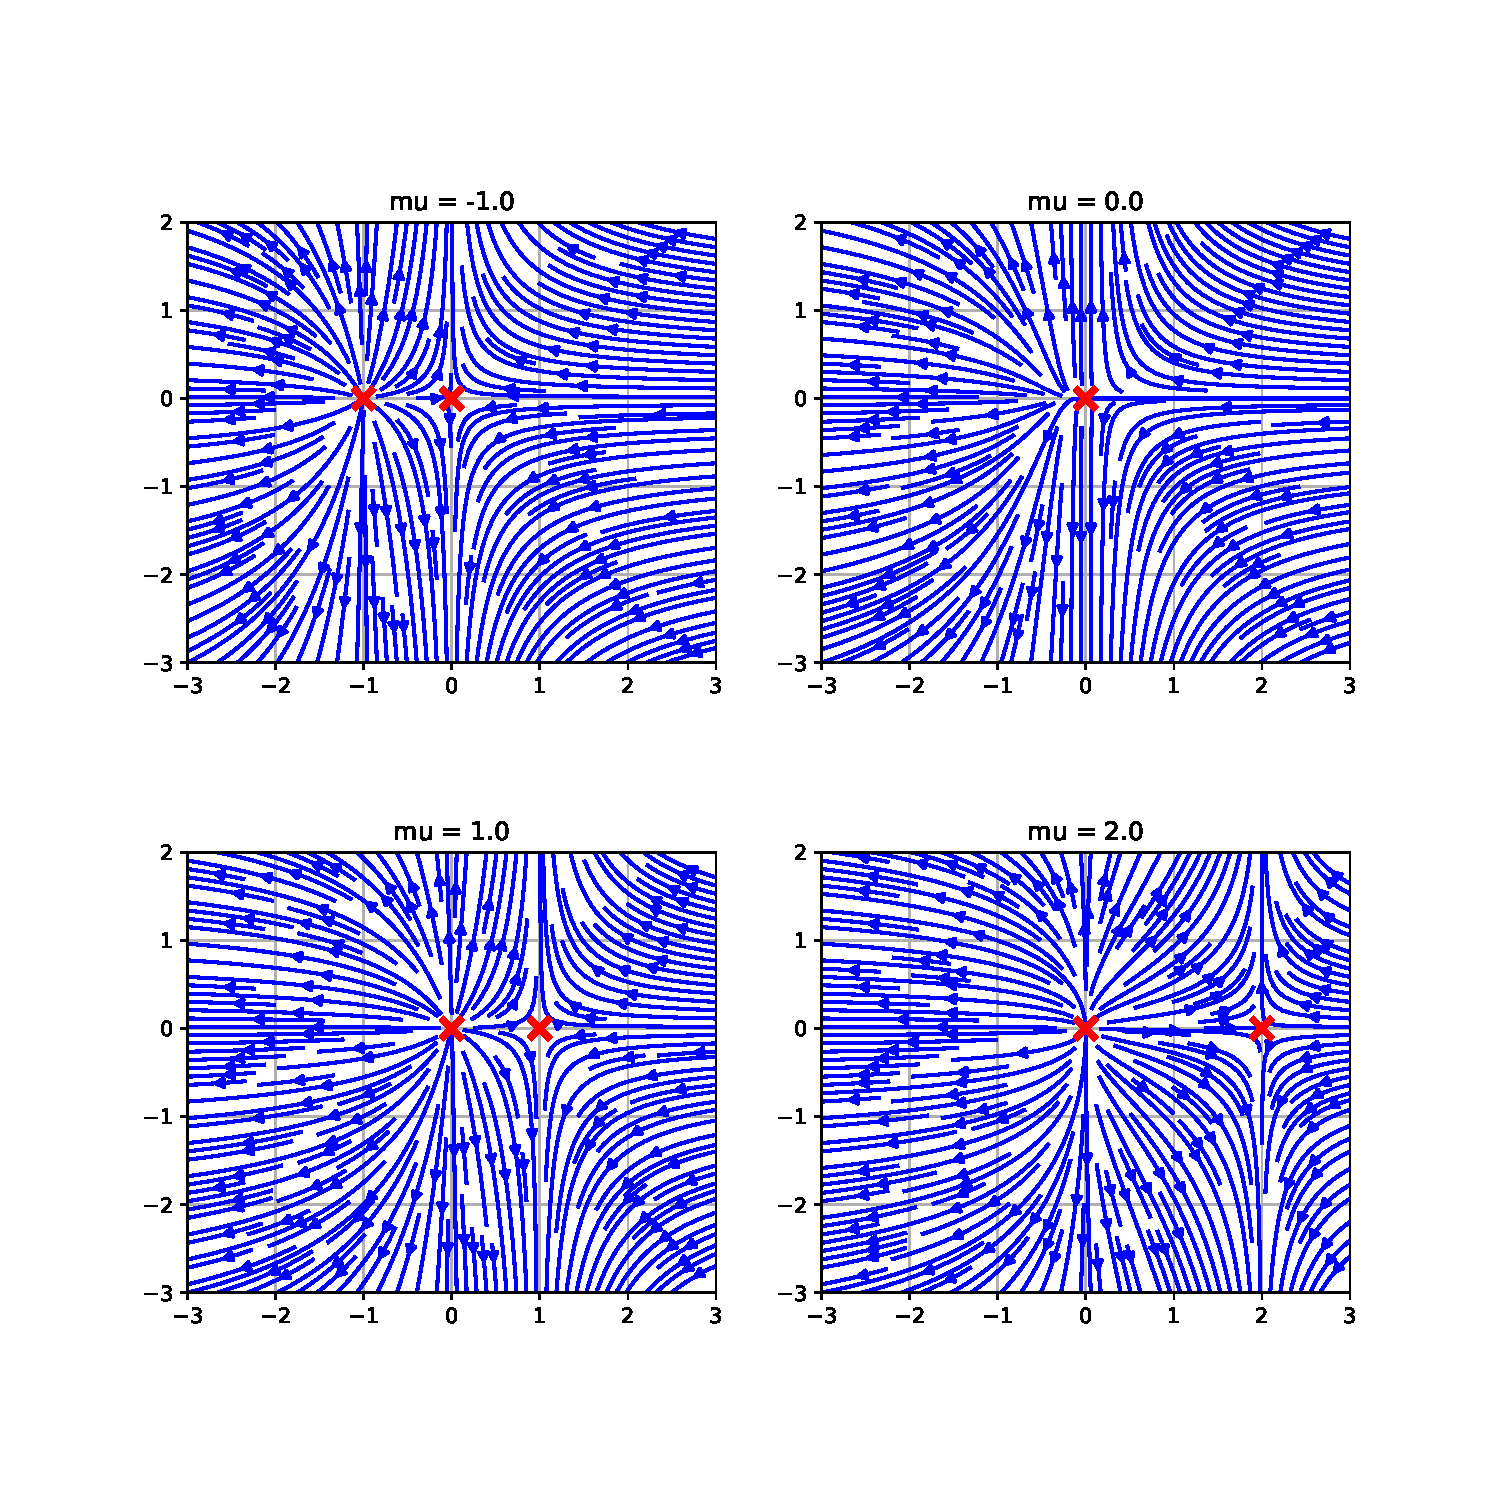
\includegraphics[width=\textwidth]{images/test/problem_1a.pdf}
    \caption{Фазовий портрет для системи з задачі $1(a)$. \textcolor{blue}{Синім} показано траєкторії руху точок, а \textcolor{red}{червоним} -- точки спокою.}
    \label{fig:problem_1a}
\end{figure}

\textbf{Пункт (б).} Так само розглядаємо три випадки.

\textit{Випадок 1. $\mu < 0$.} Точок спокою немає, оскільки $\mu - x^2 = 0$ не має розв'язків над $\mathbb{R}$. 

\textit{Випадок 2. $\mu=0$.} Точка спокою одна -- $(0,0)$ і система набуває аналогічного виду, як для випадку $\mu=0$ у пункті (а).

\textit{Випадок 3. $\mu > 0$.} Тут маємо дві точки спокою: $(\sqrt{\mu},0)$ та $(-\sqrt{\mu},0)$. Причому, $(-\sqrt{\mu},0)$ є нестійкою, а ось $(\sqrt{\mu},0)$ є стійкою. На картинці це буде відповідати сідлу для $(\sqrt{\mu},0)$ та нестійкому вузлу для $(-\sqrt{\mu}, 0)$. 

Наше передбачення перевіримо на рисунку \ref{fig:problem_1b}. Дійсно, для $\mu=-1$ точок спокою немає, відбувається ``течія'' вліво. Для $\mu=0$ бачимо той самий малюнок, як і для випадку $\mu=0$ у пункті (а). Нарешті, для $\mu=1$ та $\mu=2$ маємо дві точки спокою $(\pm\sqrt{\mu}, 0)$, де зліва нестійкий вузол, а праворуч -- сідло.

\begin{figure}
    \centering
    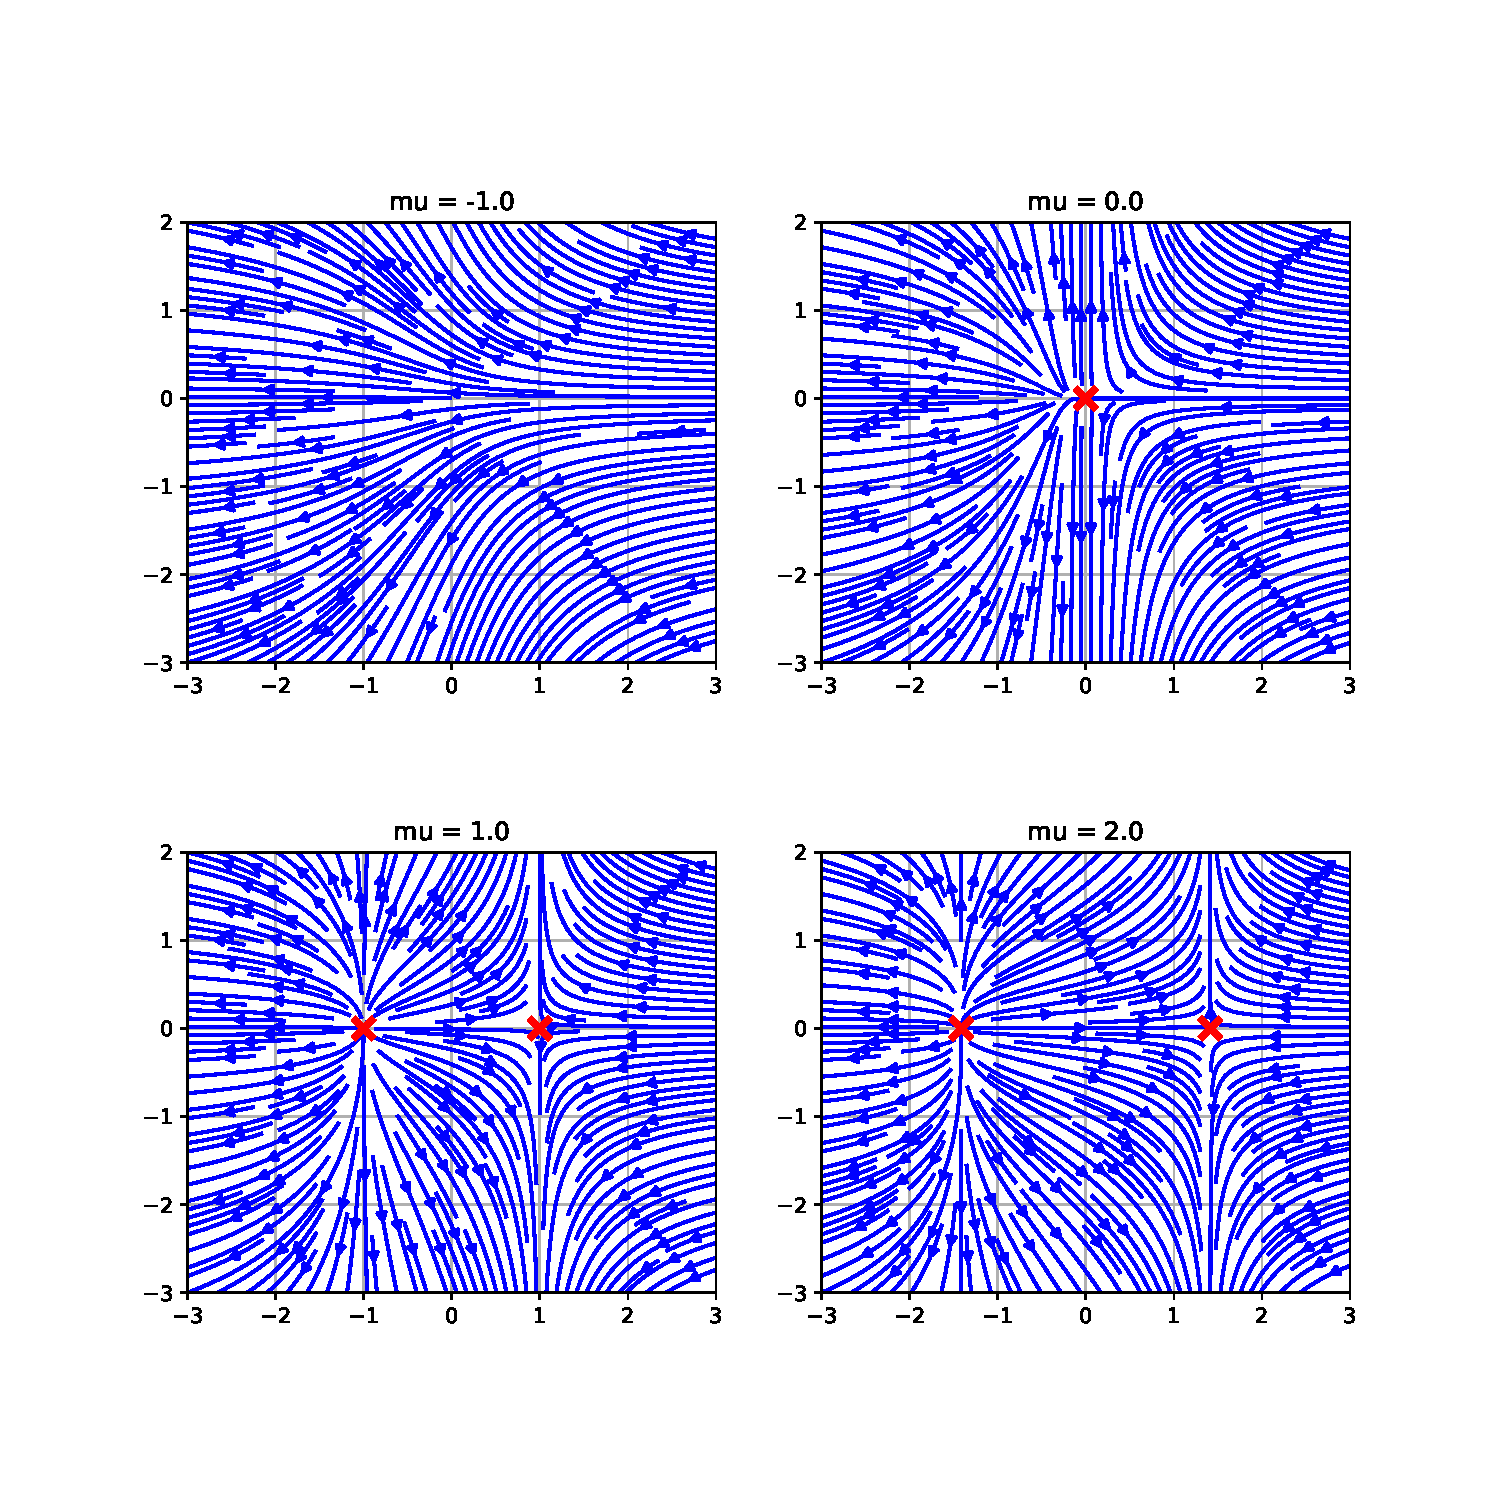
\includegraphics[width=\textwidth]{images/test/problem_1b.pdf}
    \caption{Фазовий портрет для системи з задачі $1(\text{б})$. \textcolor{blue}{Синім} показано траєкторії руху точок, а \textcolor{red}{червоним} -- точки спокою.}
    \label{fig:problem_1b}
\end{figure}

\pagebreak
\textbf{Опис зміни через нуль.} 

\textit{Пункт (а).} При переході з $\mu=\mu_- < 0$ на $\mu=\mu_+ > 0$, дві точки спокою (нестійкий вузол та сідло) спочатку вироджуються у одну (напіввузол і напівсідло), а далі ``змінюються'' ролями -- таким чином, зліва завжди вузол, а праворуч -- сідло.

\textit{Пункт (б).} При переході з $\mu=\mu_- < 0$ на $\mu=\mu_+ > 0$, спочатку точок спокою немає, далі з'являється одна, а далі вироджується дві точки: сідло і нестійкий вузол.

\textbf{Код на Python.} Знизу, наводимо текст програми для генерації картинок для обох пунктів задачі. 

\begin{lstlisting}[language=Python]
import numpy as np
import matplotlib.pyplot as plt

from typing import Callable, Tuple, List

def gen_streamplot_params(f: Callable[[float], callable], mu: float = 1.0) -> List[np.ndarray]:
    """
    Based on the vector field parameterization function and mu parameter provided, 
    generates the meshgrid and vector field needed to build the streamplot.
    
    Args:
    - `f` - the vector field function parameterization. Returns the callable vector field function
    based on the mu parameter provided.
    - `mu` - the mu parameter in the system of ODEs
    
    Output:
    - `[xx, yy, f1, f2]` - a list of numpy arrays needed to build the streamplot (x, y) coordinates
    and the corresponding vector field (f1, f2)
    """

    x = np.linspace(-3.0, 3.0, 50)  
    y = np.linspace(-3.0, 2.0, 50)  
    xx, yy = np.meshgrid(x,y)
    f = f(mu) # Choosing correct vector field function based on mu
    f1, f2 = f(xx,yy)
    return [xx, yy, f1, f2]

def draw_streamplot(ax: plt.axes, 
                    f: callable, 
                    stationary_points: List[Tuple[float, float]] = [], 
                    mu: float = 1.0) -> None:
    """
    Draws a streamplot on the provided axes based on the mu parameter and vector field provided.
    
    Args:
    - `ax` - the axes object to draw the streamplot on
    - `f` - the vector field function
    - `stationary_points` - a list of stationary points to be marked on the plot. Empty by default.
    - `mu` - the mu parameter in the system of ODEs
    
    Output:
    `None`, modifies the provided ax
    """
    
    # Some fancy customizations
    ax.set_aspect('equal')
    ax.grid()
    ax.set_title(f'mu = {mu}')
    
    # Drawing the streamplot
    xx, yy, f1, f2 = gen_streamplot_params(f, mu=mu)
    ax.streamplot(xx, yy, f1, f2, density=1.8, color='b')
    
    # Drawing the stationary points
    for point in stationary_points:
        ax.scatter(point[0], point[1], color='red', marker='x', alpha=1.0, s=100, linewidths=3.0, zorder=10)
    

if __name__ == '__main__':
    # Defining the vector field function for problem (a)
    def fn_problem_a(mu: float) -> callable:
        def fn(x: np.ndarray, y: np.ndarray) -> np.ndarray:
            return mu*x - x**2, y
        
        return fn
    
    # Defining the vector field function for problem (b)
    def fn_problem_b(mu: float) -> callable:
        def fn(x: np.ndarray, y: np.ndarray) -> np.ndarray:
            return mu - x**2, y
        
        return fn
    
    # Plotting problem (a)
    fig, axs = plt.subplots(2, 2)
    fig.set_figheight(10)
    fig.set_figwidth(10)
    
    draw_streamplot(axs[0, 0], fn_problem_a, stationary_points=[(-1.0, 0.0), (0.0, 0.0)], mu=-1.0)
    draw_streamplot(axs[0, 1], fn_problem_a, stationary_points=[(0.0, 0.0)], mu=0.0)
    draw_streamplot(axs[1, 0], fn_problem_a, stationary_points=[(1.0, 0.0), (0.0, 0.0)], mu=1.0)
    draw_streamplot(axs[1, 1], fn_problem_a, stationary_points=[(2.0, 0.0), (0.0, 0.0)], mu=2.0)
    fig.savefig(f'problem_1a.pdf')
    
    # Plotting problem (b)
    fig, axs = plt.subplots(2, 2)
    fig.set_figheight(10)
    fig.set_figwidth(10)
    
    draw_streamplot(axs[0, 0], fn_problem_b, mu=-1.0)
    draw_streamplot(axs[0, 1], fn_problem_b, stationary_points=[(0.0, 0.0)], mu=0.0)
    draw_streamplot(axs[1, 0], fn_problem_b, stationary_points=[(-1.0, 0.0), (1.0, 0.0)], mu=1.0)
    draw_streamplot(axs[1, 1], fn_problem_b, stationary_points=[(-np.sqrt(2.0), 0.0), (np.sqrt(2.0), 0.0)], mu=2.0)
    fig.savefig(f'problem_1b.pdf')
\end{lstlisting}

\problem{Полярні координати.}
\hspace{20px}\textbf{Умова.} Нарисуйте фазовий портрет наступної системи, записаної у полярних координатах:
\begin{equation}
    \begin{cases}
        \dot{r} = r(1-r) \\
        \dot{\varphi} = \sin \varphi
    \end{cases}
\end{equation}

\textbf{Розв'язання.} Напевно, цікавіше буде одразу подивитися на портрет і побачити особливості, що ми будемо обгрунтовувати. Отже, портрет зображено на Рис. \ref{fig:problem_2}. Для його побудови, ми взяли випадковим чином 50 точок всередині $r=1$ та 50 точок за кругом (код наведений в кінці).

\begin{figure}
    \centering
    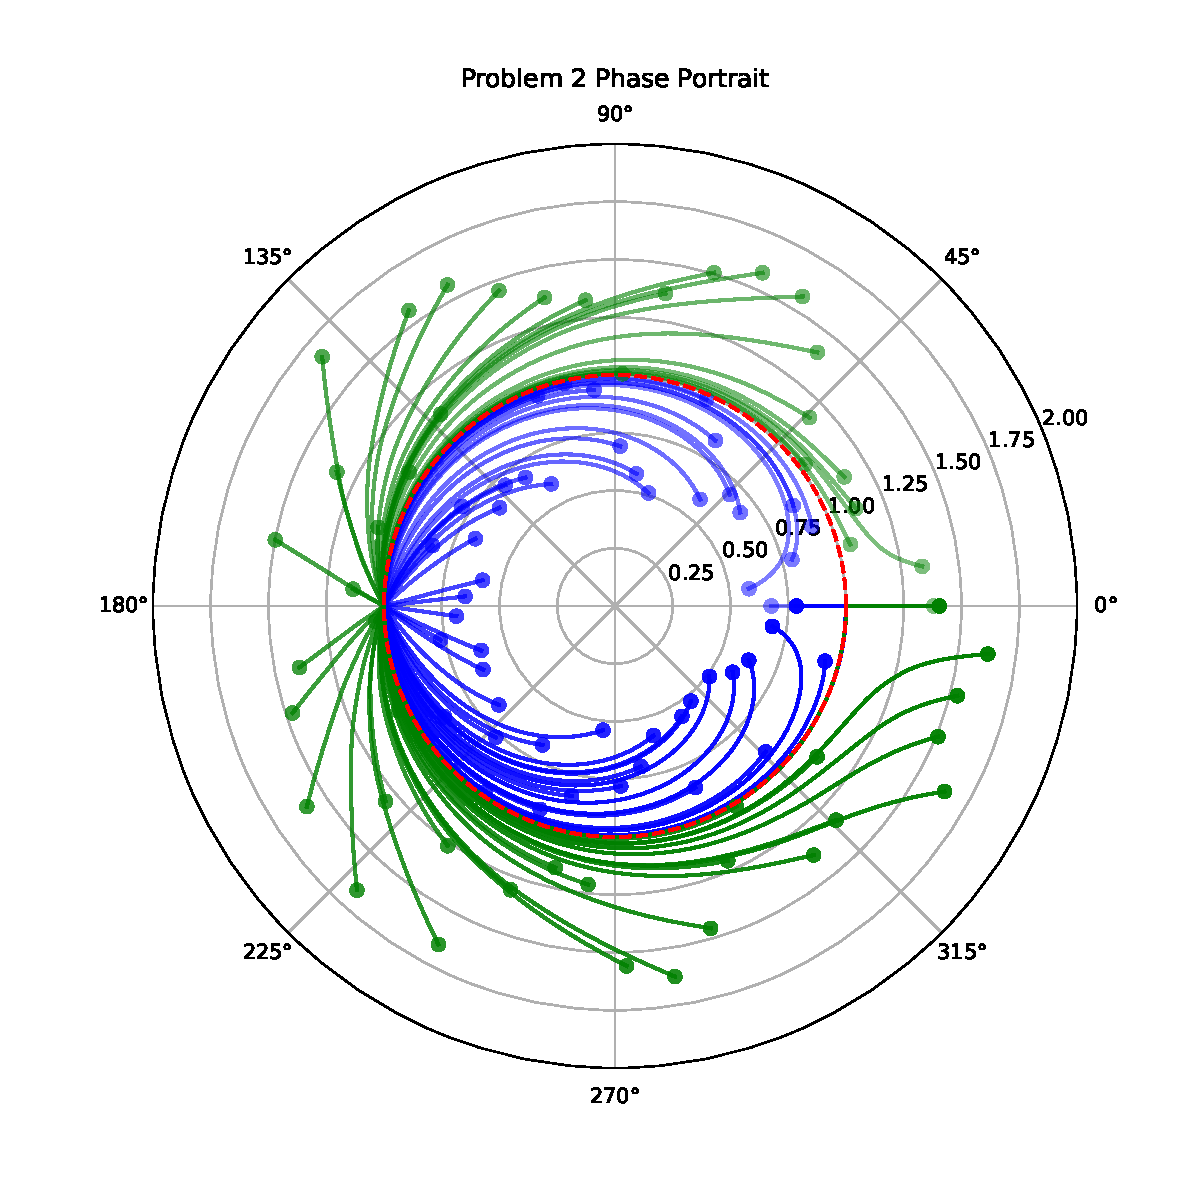
\includegraphics[width=\textwidth]{images/test/problem_2.pdf}
    \caption{Фазовий портрет для системи з задачі $2$. \textcolor{blue}{Синім} показано траєкторії руху точок, котрі починають рух всередині круга $r=1$, а \textcolor{green}{зеленим} -- за кругом.}
    \label{fig:problem_2}
\end{figure}

Бачимо дуже цікаву поведінку: усі точки, де б вони не почали свій рух, наближаються до точки з координатою $(1,\pi)$. Причому, під час руху, ці точки часто встигають ``накрутитися'' на коло $r=1$. Але чому так відбувається?

По-перше, знайдемо стаціонарні точки системи: це $(r,\varphi)=(0,\pi k)$ та $(r,\varphi)=(1,\pi k)$, де $k \in \mathbb{Z}$. На полярному графіку це відповідає трьом точкам $(0,0), (1,0), (1,\pi)$. Як видно з малюнку, $(1,\pi)$ виглядає як стійка точка, а $(0,0)$ та $(1,\pi)$ як нестійкі. Але як це можна побачити?

Проаналізуємо рівняння. Рівняння $\dot{r}=r(1-r)$ та $\dot{\varphi}=\sin\varphi$ можна розв'язувати окремо. Почнемо з першого: подивимось, як буде поводити себе функція $r(t)$ при початковій умові $r(0)=r_0$.

Якщо $r_0=0$, то точка просто буде постійно в нулі, але при дуже малій зміні $r_0$ (тобто коли $r_0 \in (0,1)$) почне стрімко віддалятись до $r=1$. Так само для точок $r_0>1$ -- вони будуть наближатися до кола $r=1$, оскільки швидкість буде завжди від'ємна. Нарешті, випадок $r_0=1$ відповідає тому, що точка увесь час буде рухатись вздовж кола $r=1$. Можна подумати, що при цьому $r=1$ буде стійким циклом, але це не зовсім так через друге рівняння $\dot{\varphi} = \sin \varphi$. 

Тепер розглянемо друге рівняння. Зафіксуємо $\varphi(0)=\varphi_0 \in [0,2\pi)$. Спочатку нехай $\varphi_0 \in (0,\pi)$. В такому разі $\sin \varphi_0>0$ і тому кут почне збільшуватись. Збільшуватись він буде асимптотично до значення $\varphi=\pi$. Якщо ж $\varphi_0 \in (\pi,2\pi)$, то швидкість $\sin \varphi_0 < 0$ і тому кут почне зменьшуватись, знову ж таки, до $\varphi=\pi$. Нарешті, якщо або $\varphi=0$, або $\varphi=\pi$, то точка буде залишатись на відповідному промені увесь час (тільки промінь $\varphi=0$ свого роду нестабільний, а $\varphi=\pi$ -- стабільний). 

Тому, радіально траєкторії будуть наближатися до кола $r=1$, але потім по куту ``з'їжджати'' до $\varphi=\pi$.

\textbf{Код на Python.} 
\begin{lstlisting}[language=Python]
import numpy as np
import matplotlib as mpl
import matplotlib.pyplot as plt
import random
from scipy.integrate import solve_ivp

if __name__ == '__main__':
    fig = plt.figure(figsize=(8, 8))
    ax = fig.add_subplot(polar=True)

    plt.xlim([0, 2*np.pi])  
    plt.ylim([0, 1.5])  

    def f(_t, x):
        return x[0]*(1-x[0]), np.sin(x[1])

    N = 1000
    T = 60
    t = np.linspace(0, T, N)

    POINTS_NUMBER = 50
    
    # Points inside r = 1
    for i, phi in enumerate(np.linspace(0, 2*np.pi, POINTS_NUMBER)):
        x0 = [0.5 + 0.5 * random.random(), phi]
        res = solve_ivp(f, [0, T], x0, dense_output=True)
        s = res.sol(t)
        
        # Drawing
        alpha = 0.5 + 0.5 * i / len(np.linspace(0, 2*np.pi, POINTS_NUMBER))
        ax.plot(s[1], s[0], color='blue', alpha=alpha)
        ax.plot(x0[1], x0[0], color='blue', marker='o', alpha=alpha)
    
    # Points outside r = 1
    for i, phi in enumerate(np.linspace(0, 2*np.pi, POINTS_NUMBER)):
        x0 = [1.0 + 0.75 * random.random(), phi]
        res = solve_ivp(f, [0, T], x0, dense_output=True)
        s = res.sol(t)
        
        # Drawing
        alpha = 0.5 + 0.5 * i / len(np.linspace(0, 2*np.pi, POINTS_NUMBER))
        ax.plot(s[1], s[0], color='green', alpha=alpha)
        ax.plot(x0[1], x0[0], color='green', marker='o', alpha=alpha)
    
    # Some customizations
    ax.set_rmax(1.5)
    ax.set_rticks([0.25, 0.5, 0.75, 1, 1.25, 1.5, 1.75, 2.0])
    ax.grid(True)
    ax.plot(np.linspace(0, 2*np.pi, N), np.ones(N), color='red', linestyle='dashed')
    mpl.rcParams['figure.dpi'] = 600 
    ax.set_title("Problem 2 Phase Portrait", va='bottom') 
    plt.savefig('problem_2.pdf')    
\end{lstlisting}

\end{document}
